\documentclass[tikz,border=5]{standalone}
\usepackage{amsmath}
\usepackage{amssymb}
\usepackage{amsmath,amsthm,amssymb,amscd}
\usepackage{xcolor}
\usepackage{tikz}
\usepackage{pgfplots}
\pgfplotsset{compat=newest}
\usepgfplotslibrary{groupplots}
\usepgfplotslibrary{dateplot}
\tikzset{
  causalvar/.style      = {draw, circle, node distance = 2cm}
}
\usepackage{amsmath}
\usetikzlibrary{matrix}
\usetikzlibrary{shapes,arrows}
\usepackage{amsmath}
\usepackage{amsmath,amsthm,amssymb,amscd}
\usepackage{xcolor}
\usepackage{tikz}
\usepackage{pgfplots}
\pgfplotsset{compat=newest}
\usepgfplotslibrary{groupplots}
\usepgfplotslibrary{dateplot}
\tikzset{
  causalvar/.style      = {draw, circle, node distance = 2cm}
}
\usetikzlibrary{matrix}
\usetikzlibrary{shapes,arrows}
\usepackage{amssymb}

\begin{document}

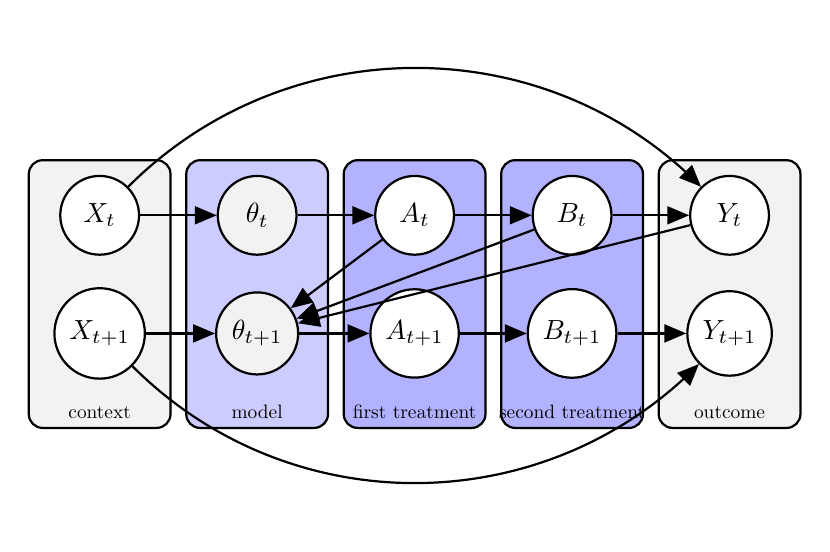
\begin{tikzpicture}[auto, thick, node distance=1cm, >=triangle 45]
%,->,>=stealth',auto,node distance=3cm,
\tikzstyle{unobserved}=[thick, dashed, fill=gray!0]
\tikzstyle{squared}=[thick, fill=gray!10, rounded corners=5pt]
\tikzstyle{norn}=[thick, fill=gray!0, minimum size=1cm]
\draw[squared] (-2.9,-2.7) rectangle (-1.1,0.7);
\draw[squared, fill=blue!20] (-0.9,-2.7) rectangle (0.9,0.7);
\draw[squared, fill=blue!30] (1.1,-2.7) rectangle (2.9,0.7);
\draw[squared, fill=blue!30] (3.1,-2.7) rectangle (4.9,0.7);
\draw[squared] (5.1,-2.7) rectangle (6.9,0.7);
\draw
	node[norn] at (2,0)[causalvar](A){$A_t$}
	node[norn] at (4,0)[causalvar](B){$B_t$}
	node[norn] at (6,0)[causalvar](Y){$Y_t$}
        node[norn] at (6,-1.5)[causalvar](Yp){$Y_{t+1}$}
	node[norn] at (-2,0)[causalvar](X){$X_t$}
        node[norn] at (-2,-1.5)[causalvar](Xp){$X_{t+1}$}
    node[squared, minimum size=1cm] at (0,0)[causalvar](theta_t){$\theta_t$}
    node[squared] at (0,-1.5)[causalvar](theta_t_p){$\theta_{t+1}$}
    node[norn] at (2,-1.5)[causalvar](A2){$A_{t+1}$}
    node[norn] at (4,-1.5)[causalvar](B2){$B_{t+1}$};
    ;
	
\draw (0,-2.5)node[scale=0.7]{model};
\draw (2,-2.5)node[scale=0.7]{first treatment};
\draw (-2.,-2.5)node[scale=0.7]{context};
\draw (4,-2.5)node[scale=0.7]{second treatment};
\draw (6,-2.5)node[scale=0.7]{outcome};
	\draw[->](X) --  (theta_t) node[midway, near end] {};
    \draw[->](theta_t) to node {} (A);
	\draw[->](A) to node {} (B);
	\draw[->](B) to node {} (Y);
	\draw[->](X) to [out=45,in=135] node {} (Y);
        \draw[->](Xp) to [out=-45,in=-135] node {} (Yp);
    \draw[->](Xp) --  (theta_t_p) node[midway, near end] {};
    \draw[->](theta_t_p) to node {} (A2);
    \draw[->](A2) to node {} (B2);
    \draw[->](B2) to node {} (Yp);
    \draw[->](A) to node {} (theta_t_p);
    \draw[->](B) to node {} (theta_t_p);
    \draw[->](Y) to node {} (theta_t_p);
\end{tikzpicture}

\end{document}